\documentclass[a4paper,10pt]{article}
\usepackage[utf8]{inputenc}
\usepackage[spanish]{babel}
\usepackage[affil-it]{authblk}
\usepackage{enumerate}
\usepackage{graphicx}
\usepackage{hyperref}
\usepackage{amsmath}
\usepackage{amssymb}
\usepackage{cancel}
\usepackage[usenames, dvipsnames]{color}
\usepackage{tikz}
\usepackage[labelfont=bf]{caption}
\usepackage{subcaption} %Multiple images
\usepackage{multicol} % Multiple columns
\usepackage{float}
\usepackage{cleveref}
 \usepackage{relsize} % bigger math symbols
\usepackage[margin=1.4in]{geometry}
\usepackage[titletoc,toc,title]{appendix}
\usepackage{enumitem}
\usepackage{etoolbox}
\usepackage{mdframed} %frame theorems
\usetikzlibrary{calc}
\numberwithin{equation}{section}

% Enviroment for theorems
\newmdtheoremenv[frametitle=Teorema]{theo}{Theorem}

% Circled words
\newcommand{\circled}[2][]{%
  \tikz[baseline=(char.base)]{%
    \node[shape = circle, draw, inner sep = 1pt]
    (char) {\phantom{\ifblank{#1}{#2}{#1}}};%
    \node at (char.center) {\makebox[0pt][c]{#2}};}}
\robustify{\circled}

%Appendices in spanish
\renewcommand{\appendixname}{Ap\'endices}
\renewcommand{\appendixtocname}{Ap\'endices}
\renewcommand{\appendixpagename}{Ap\'endices}

%Zero delimiter
\newcommand{\zerodel}{.\kern-\nulldelimiterspace}

%Columns separation
\setlength{\columnsep}{1cm}

%Indentation
\setlength{\parindent}{0ex}

%Multiple References

\crefrangelabelformat{equation}{(#3#1#4--#5\crefstripprefix{#1}{#2}#6)}

\usepackage{xparse}

%Boxes

\newcommand*{\boxcolor}{blue}
\makeatletter
\renewcommand{\boxed}[1]{\textcolor{\boxcolor}{%
\tikz[baseline={([yshift=-1ex]current bounding box.center)}] \node [rectangle, minimum width=1ex,rounded corners,draw] {\normalcolor\m@th$\displaystyle#1$};}}
 \makeatother

%Constantes
\newcommand{\euler}{\mathrm{e}}
\newcommand{\im}{i}

%Lemas, teoremas, definiciones y pruebas
\newcommand{\definicion}{\textbf{Definición: }}
\newcommand{\lema}{\textbf{Lema: }}
\newcommand{\teorema}{\textbf{Teorema: }}
\newcommand{\prueba}{\textbf{Prueba: }}
\newcommand{\proposicion}{\textbf{Proposición: }}
\newcommand{\corolario}{\textbf{Corolario: }}

% Definición de las secciones y su numeración

\makeatletter
\def\@seccntformat#1{%
  \expandafter\ifx\csname c@#1\endcsname\c@section\else
  \csname the#1\endcsname\quad
  \fi}
\makeatother

%opening
\title{Mecánica Clásica Tarea \# 15}
\author{Favio Vázquez\thanks{Correo: favio.vazquezp@gmail.com}}\affil{Instituto de Ciencias Nucleares. Universidad Nacional Autónoma de México.}
\date{}

\begin{document}

\makeatletter
\def\@maketitle{%
  \newpage
  \null
  \vskip 2em%
  \begin{center}%
  \let \footnote \thanks
    {\Large\bfseries \@title \par}%
    \vskip 1.5em%
    {\normalsize
      \lineskip .5em%
      \begin{tabular}[t]{c}%
        \@author
      \end{tabular}\par}%
    \vskip 1em%
    {\normalsize \@date}%
  \end{center}%
  \par
  \vskip 1.5em}
\makeatother

\maketitle

\textbf{NOTA}: En los billares hay trayectorias que son singulares que son aquellas
en las que la partícula llega a incidir exactamente en uno de los vértices. Desprecie 
esta posibilidad limitando sus cálculos al conjunto de trayectorias no singulares.

\vspace{.3cm}

\section{Problema 1}

Una partícula de masa $m$ se mueve libremente en el interior de un rectángulo de 
lados $a$ y $b$ y rebota elásticamente al incidir sobre los lados del rectángulo 
(billar). Encuentre, si es que existen, unas coordenadas o variables de acción 
y ángulo para este sistema. A partir de estas variables encuentre, si es que existen,
las frecuencias asociadas al movimiento. 

\vspace{.3cm}

\underline{Solución:} \vspace{.3cm}

\section{Problema 2}

Encuentre coordenadas de acción y ángulo para el péndulo esférico (puede dejar 
indicadas algunas integrales). Trace figuras, similares a las que se trazaron 
en clase para el problema de Kepler, en las que se muestra que las trayectorias 
están sobre toros de dos dimensiones inmersos en el espacio fase de cuatro. 
(Use la computadora para hacer las figuras).

\vspace{.3cm}

\underline{Solución:} \vspace{.3cm}

Recordemos que las coordenadas de acción y ángulo existen sólo en las regiones 
acotadas del espacio de fase de un sistema integrable, y que estas son 
coordenadas canónicas en las que los impulsos son integrales de movimiento y 
determinan a uno de los toros y las coordenadas conjugadas de estos impulsos 
son ángulos que determinan a un punto de dicho toro. Por lo tanto es necesario 
demostrar que el péndulo esférico es un sistema integrable, y encontrar las 
coordenadas de ángulo y acción para su espacio de fases que será acotado. 

\vspace{.3cm}

Debajo se encuentra un diagrama del péndulo esférico,

\begin{figure}[H]
 \center 
 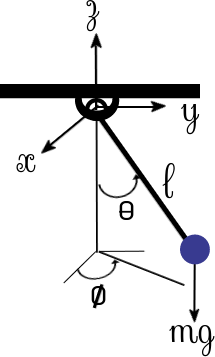
\includegraphics[scale=0.6]{problema2fig1}
 \caption{Péndulo esférico.}
 \label{fig:problema2fig1}
\end{figure}

recordamos que para el péndulo esférico la lagrangiana se escribe como 

\begin{equation}
 L = T - V = \frac{1}{2}ml^2(\dot{\theta}^2 + \dot{\phi}^2\sen^2{\theta}) 
 - mgl\cos{\theta},
\end{equation}

podemos ahora escribir la hamiltoniana del sistema, primero obteniendo los momentos 
conjugados para las variables $\theta$ y $\phi$, 

\begin{equation}
 p_\theta = \frac{\partial L}{\partial \dot{\theta}} = ml^2\dot{\theta},
\end{equation}

\begin{equation}
 p_\phi = \frac{\partial L}{\partial \dot{\phi}} = ml^2\dot{\phi}\sen^2{\theta},
\end{equation}

de donde obtenemos 

\begin{equation}
 \dot{\theta} = \frac{p_\theta}{ml^2},
\end{equation}

y

\begin{equation}
 \dot{\phi} = \frac{p_\phi}{ml^2\sen^2{\theta}},
\end{equation}

y ahora utilizando 

\begin{equation}
 H = \sum_i p_i \dot{q}^2(q,p) - L, 
\end{equation}

la hamiltoniana del péndulo esférico resulta

\begin{equation}
 H = \frac{p_\theta^2}{2ml^2} + \frac{p_\phi^2}{2ml^2\sen^2{\theta}} 
 + mgl\cos{\theta}.
 \label{eq:hamiltonianaPendEsf}
\end{equation}

Podemos notar ahora dos cosas. Primero, debido a que la coordenada $\phi$ es 
ignorable según la forma de la lagrangiana, entonces su momento conjugado se 
conservará, es decir que $p_\phi$ es constante y es una integral de movimiento,
y además debido a que la energía  cinética es una forma cuadrática de las 
velocidades y que la lagrangiana no depende explícitamente del tiempo,
entonces la hamiltoniana es igual a la energía total  del sistema, que también
será una integral de movimiento. Usando la notación del método de Liouville, 
podemos escribir esto de la siguiente forma 

\begin{equation}
  \frac{p_\theta^2}{2ml^2} + \frac{p_\phi^2}{2ml^2\sen^2{\theta}} 
 + mgl\cos{\theta} = I_1 = E,
 \label{eq:energiaPendEsf}
\end{equation}

\begin{equation}
 p_\phi = I_2.
 \label{eq:pphiPendEsf}
\end{equation}

Ahora hemos encontrado entonces dos integrales de movimiento, nos preguntamos ahora 
si están en involución, es decir si 

\begin{equation}
 \{I_1, I_2\} = 0,
\end{equation}

para ver esto recordamos la expresión para los paréntesis de Poisson, 

\begin{equation}
 \frac{\partial I_1}{\partial \theta}\cancelto{0}{\frac{I_2}{\partial p_\theta}} 
 - \frac{\partial I_1}{\partial p_\theta}\cancelto{0}{\frac{I_2}{\partial \theta}} + 
 \cancelto{0}{\frac{\partial I_1}{\partial \phi}}\frac{I_2}{\partial p_\phi} 
 - \frac{\partial I_1}{\partial p_\phi}\cancelto{0}{\frac{I_2}{\partial \phi}} = 
 0.
\end{equation}

Por lo tanto hemos demostrado que las dos integrales de movimiento que hemos encontrado 
están en involución, y debido a que hay tantas integrales de movimiento en involución como grados 
de libertad el sistema es integrable y podemos proceder a encontrar las coordenadas de 
acción y ángulo. Para hacer esto comenzamos escribiendo la ecuación de Hamilton-Jacobi 
a partir de la hamiltoniana \eqref{eq:hamiltonianaPendEsf}, 

\begin{equation}
 \frac{1}{2ml^2}\left(\frac{\partial G}{\partial \theta} \right)^2 
 + \frac{1}{2ml^2\sen^2{\theta}}\left(\frac{\partial G}{\partial \phi} \right)^2 
 + mgl\cos{\theta} = - \frac{\partial G}{\partial t}.
\end{equation}

Proponemos ahora la siguiente solución para la $G$, 

\begin{equation}
 G(\theta,\phi,t) = W(\theta,\phi) +  T(t),
\end{equation}

y entonces 

\begin{equation}
 \frac{1}{2ml^2}\left(\frac{\partial W}{\partial \theta} \right)^2 
 + \frac{1}{2ml^2\sen^2{\theta}}\left(\frac{\partial W}{\partial \phi} \right)^2 
 + mgl\cos{\theta} = - \frac{\partial T}{\partial t}.
\end{equation}

Como el lado izquierdo de esta ecuación depende solamente de $\theta$ y $\phi$ y el 
derecho del tiempo, ambos términos deben ser iguales a misma constante que llamaremos 
$\alpha_1$, y tenemos que 

\begin{equation}
 \frac{\partial T}{\partial t} = - \alpha_1 \Rightarrow 
 T(t) = - \alpha_1 t,
\end{equation}

donde hemos hecho cero la constante aditiva de integración ya que no afectará la 
solución final, y también nos queda que 

\begin{equation}
 \frac{1}{2ml^2}\left(\frac{\partial W}{\partial \theta} \right)^2 
 + \frac{1}{2ml^2\sen^2{\theta}}\left(\frac{\partial W}{\partial \phi} \right)^2 
 + mgl\cos{\theta} = \alpha_1,
\end{equation}

y ahora proponemos que $W$ puede separase en una parte que depende sólo de $\theta$ 
y otra que solo depende de $\phi$, i.e. 

\begin{equation}
 W(\theta,\phi) = W_\theta(\theta) + W_\phi(\phi),
\end{equation}

y al sustituir esto en la ecuación para $W$ obtenemos 

\begin{equation}
 \frac{1}{2ml^2}\left[\left(\frac{\partial W_\theta}{\partial \theta} \right)^2 
 + \frac{1}{\sen^2{\theta}}\left(\frac{\partial W_\phi}{\partial \phi} \right)^2\right]
 + mgl\cos{\theta} = \alpha_1.
\end{equation}

De esta ecuación vemos que la dependencia en $\phi$ solo se encuentra en el término 
$(\partial W_\phi/\partial \phi)^2$ por lo tanto este debe ser igual a una constante 
que llamaremos $\alpha_2$, por lo tanto 

\begin{equation}
 \left(\frac{\partial W_\phi}{\partial \phi}\right)^2 = \alpha_2 \Rightarrow 
 W_\phi(\phi) = \sqrt{\alpha_2}\phi,
\end{equation}

y

\begin{equation}
 \frac{1}{2ml^2}\left[\left(\frac{\partial W_\theta}{\partial \theta} \right)^2 
 + \frac{\alpha_2^2}{\sen^2{\theta}}\right]
 + mgl\cos{\theta} = \alpha_1.
\end{equation}

De esta ecuación podemos obtener $W_\theta$, para esto despejamos 
$\partial W_\theta/\partial \theta$,

\begin{equation}
 \frac{\partial W_\theta}{\partial \theta} = \pm \left[
 2ml^2(\alpha_1 - mgl\cos{\theta}) -  \alpha_2^2\csc^2{\theta}\right]^{1/2},
\end{equation}

\begin{equation}
 \therefore W_\theta = \int \pm \left[
 2ml^2(\alpha_1 - mgl\cos{\theta}) -  \alpha_2^2\csc^2{\theta}\right]^{1/2} d\theta,
\end{equation}

y entonces 

\begin{equation}
 W(\theta,\phi) = \sqrt{\alpha_2}\phi + \int \pm \left[
 2ml^2(\alpha_1 - mgl\cos{\theta}) -  \alpha_2^2\csc^2{\theta}\right]^{1/2} d\theta,
\end{equation}

y 

\begin{equation}
 \boxed{G(\theta,\phi,t) = \sqrt{\alpha_2}\phi + \int \pm \left[
 2ml^2(\alpha_1 - mgl\cos{\theta}) -  \alpha_2^2\csc^2{\theta}\right]^{1/2} d\theta 
 - \alpha_1 t.}
\end{equation}

Calculemos ahora entonces los momentos con las relaciones de Hamilton-Jacobi, 

\begin{equation}
 p_i = \frac{\partial G}{\partial q^i},
\end{equation}

con lo que obtenemos lo ya sabíamos sobre $p_\phi$, i.e. que es constante, 

\begin{equation}
 p_\phi = \frac{\partial G}{\partial \phi} = \sqrt{\alpha_2},
\end{equation}

y para $p_\theta$, 

\begin{equation}
 p_\theta = \frac{\partial G}{\partial \theta} = \pm \left[
 2ml^2(\alpha_1 - mgl\cos{\theta}) -  \alpha_2^2\csc^2{\theta}\right]^{1/2}.
\end{equation}

Podemos ahora construir las coordenadas de acción, 

\begin{equation}
 J_i = \frac{1}{2\pi}\oint p_idq^i,
\end{equation}

que para $\phi$ será 

\begin{equation}
 J_\phi = \frac{1}{2\pi}\oint p_\phi d\phi,
\end{equation}

pero $\phi$ está acotada entre $0$ y $2\pi$, y $p_\phi = \sqrt{\alpha_2}$, entonces 

\begin{equation}
 J_\phi = \frac{\sqrt{\alpha_2}}{2\pi}\int_0^{2\pi} d\phi =  
 \frac{\sqrt{\alpha_2}}{\cancel{2\pi}}\cancel{2\pi},
\end{equation}

\begin{equation}
 \boxed{\therefore J_\phi = p_\phi = \sqrt{\alpha_2}.}
\end{equation}

Ahora para $\theta$ tenemos, 

\begin{equation}
 J_\theta = \frac{1}{2\pi}\oint \pm \left[
 2ml^2(\alpha_1 - mgl\cos{\theta}) -  \alpha_2^2\csc^2{\theta}\right]^{1/2},
\end{equation}

la cual dejaremos planteada. Ahora para las variables de ángulo usamos 

\begin{equation}
 \Theta^i = \frac{\partial}{\partial J_i}\oint \sum_k p_kdq^k,
\end{equation}

para $\phi$ esto es 

\begin{equation}
 \Theta^\phi = \frac{\partial}{\partial J_\phi}\left[ \oint p_\theta d\theta + 
 \oint p_\phi d\phi\right]
\end{equation}

\begin{equation}
 \Theta^\phi = \frac{\partial}{\partial J_\phi}\left[ \oint  
  \pm \left[2ml^2(\alpha_1 - mgl\cos{\theta}) -  
  \alpha_2^2\csc^2{\theta}\right]^{1/2}d\theta + 
  \oint \sqrt{\alpha_2} d\phi\right]
\end{equation}

\begin{equation}
 \boxed{ \Theta^\phi = \frac{\partial}{\partial J_\phi}\left[ \oint  
  \pm \left[2ml^2(\alpha_1 - mgl\cos{\theta}) -  
  \alpha_2^2\csc^2{\theta}\right]^{1/2}d\theta + 
  2\pi \alpha_2 \right].}
\end{equation}

Y para $\theta$ nos quedaría entonces 

\begin{equation}
 \boxed{ \Theta^\theta = \frac{\partial}{\partial J_\theta}\left[ \oint  
  \pm \left[2ml^2(\alpha_1 - mgl\cos{\theta}) -  
  \alpha_2^2\csc^2{\theta}\right]^{1/2}d\theta + 
  2\pi \alpha_2 \right].}
\end{equation}

Con lo cual hemos encontrado las coordenadas de acción y ángulo, dejando algunas 
integrales complicadas planteadas. Ahora para trazar las figuras similares a las 
del problema de Kepler sobre $T^2$, lo hacemos desde $p_\theta$. Es fácil ver que 
$\alpha_1$ será la energía total del péndulo esférico, y recordamos que $\alpha_2$ 
es $p_\phi$ y es constante, entonces escribimos $p_\theta$ como 

\begin{equation}
 p_\theta = \pm \left[
 2ml^2(E - mgl\cos{\theta}) -  p_\phi^2\csc^2{\theta}\right]^{1/2}.
\end{equation}

\section{Problema 3}

Una partícula de masa $m$ se mueve libremente en el interior de un triángulo  
equilátero de lado $a$ y rebota elásticamente al incidir sobre los lados del triángulo 
(billar). Encuentre, si es que existen, unas coordenadas o variables de acción 
y ángulo para este sistema. A partir de estas variables encuentre, si es que existen,
las frecuencias asociadas al movimiento. 

\vspace{.3cm}

\underline{Solución:} \vspace{.3cm}

\end{document}